\documentclass[a4paper,UTF8]{article}
\usepackage{ctex}
\usepackage[margin=1.25in]{geometry}
\usepackage{color}
\usepackage{graphicx}
\usepackage{amssymb}
\usepackage{amsmath}
\usepackage{amsthm}
\usepackage{soul, color, xcolor}
\usepackage{bm}
\usepackage{tcolorbox}
\usepackage{hyperref}
\usepackage{graphicx}
\numberwithin{equation}{section}
%\usepackage[thmmarks, amsmath, thref]{ntheorem}
\theoremstyle{definition}
\newtheorem*{solution}{Solution}
\newtheorem*{prove}{Proof}
\usepackage{multirow}
\usepackage{diagbox}
\usepackage{float}

\def \X {\mathbf{X}}
\def \A {\mathbf{A}}
\def \w {\hat{\boldsymbol{w}}}
\def \y {\mathbf{y}}
\def \x {\mathbf{x}}
\def \z {\mathbf{z}}
\def \hy {\widehat{y}}
\def \by {\Bar{y}}
\def \H {\mathbf{H}}
\def \I {\mathbf{I}}
\setlength{\parindent}{0pt}
%--

%--
\begin{document}
	\title{机器学习导论\ 习题一}
	\author{211300063, 张运吉, \href{mailto:邮箱}{211300063@smail.nju.edu.cn}}
	\maketitle
	\section*{作业提交注意事项}
	\begin{tcolorbox}
		\begin{enumerate}
			\item[1.] 请在LaTeX模板中第一页填写个人的学号、姓名、邮箱;
			\item[2.] 本次作业需提交作答后的该 pdf 文件、编程题代码(.py文件); {\color{red}\textbf{请将二者打包为~.zip 文件上传}}. 注意命名规则, 三个文件均命名为 “学号\_姓名” + “.后缀” (例如 211300001\_张三” + “.pdf”、“.py”、“.zip”);
			\item[3.] 若多次提交作业, 则在命名~.zip 文件时加上版本号, 例如 211300001\_张三\_v1.zip” (批改时以版本号最高的文件为准);
			\item[4.] 本次作业提交截止时间为 {\color{red}\textbf{ 3 月 29 日23:59:59}}. 未按照要求提交作业, 提交作业格式不正确, {\color{red}\textbf{作业命名不规范}}, 将会被扣除部分作业分数; 除特殊原因 (如因病缓交, 需出示医院假条) 逾期未交作业, 本次作业记 0 分; {\color{red}\textbf{如发现抄袭, 抄袭和被抄袭双方成绩全部取消}};
			\item[5.] 本次作业提交地址为 \href{https://box.nju.edu.cn/u/d/008080744a60484ea526/}{here}, 请大家预留时间提前上交, 以防在临近截止日期时, 因网络等原因无法按时提交作业.
		\end{enumerate}
	\end{tcolorbox}
	\newpage
	
	
	\section{[15pts] Derivatives of Matrices}
	有 $\alpha \in \mathbb{R}$, $\y\in \mathbb{R}^{m×1}$, $\x\in \mathbb{R}^{n×1}$, 试完成下题, 并给出计算过程.
	\begin{enumerate}
		\item[(1)] \textbf{[4pts]} 此问中假设 $\A\in \mathbb{R}^{n×n}$, 且 $\alpha=\x^\top\A\x$, 试求 $\frac{\partial \alpha}{\partial \x}$.
		\item[(2)] \textbf{[5pts]} 此问中假设 $\A\in \mathbb{R}^{m×n}$, 且 $\alpha=\y^\top\A\x$, 同时 $\y$、$\x$ 为 $\z$ 的函数, 试求 $\frac{\partial \alpha}{\partial \z}$.
		\item[(3)] \textbf{[6pts]} 此问中假设 $\A\in \mathbb{R}^{n×n}$ 且 $\A$ 可逆, $\A$ 为 $\alpha$ 的函数同时 $\frac{\partial \A}{\partial \alpha}$ 已知. 试求 $\frac{\partial \A^{-1}}{\partial \alpha}$.
	\end{enumerate}
	(提示: 可以参考 \href{https://www.math.uwaterloo.ca/~hwolkowi/matrixcookbook.pdf}{The Matrix Cookbook}.)
	
\begin{solution}
此处用于写解答(中英文均可) \\
\begin{enumerate}
\item[(1)]
		\begin{equation}
			A = \left[
			\begin{array}{c}
				\alpha_1^{T}  \\
				\alpha_2^{T} \\
				... \\
				\alpha_n^{T} \\
				
			\end{array}
			\right] ,   
			Ax = \left[
			\begin{array}{c}
				\alpha_1^{T}x  \\
				\alpha_2^{T}x \\
				...\\
				\alpha_n^{T}x 
			\end{array}
			\right]
		\end{equation}
		则$x^{T}Ax =  \sum\limits_{i=1}^{n}x_i\alpha_i^{T}x=a_{11}x_1^{2}+a_{12}x_1x_2+...+a_{1n}x_1x_n+a_{21}x_1x_2+a_{22}x_2^{2}+...+a_{2n}x_2x_n+...+a_{n1}x_1x_n+a_{n2}x_2x_n+...+a_{nn}x_n^{2}$
		
		$\therefore \frac{\partial \alpha}{\partial \x_k}=\sum\limits_{j=1}^{n}a_{kj}x_j+\sum\limits_{i=1}^{n}a_{ik}x_i$
          $\therefore \frac{\partial \alpha}{\partial \x}=x^{T}(A^{T}+A)$
          
\item[(2)]
	根据定义:$y^{T}Ax=\sum\limits_{i=1}^{m}\sum\limits_{j=1}^{n}a_{ij}y_ix_j$
	
	$\therefore \frac{\partial \alpha}{\partial z_k} = \sum\limits_{i=1}^{m}\sum\limits_{j=1}^{n}
	a_{ij}\left[y_i\frac{\partial x_j}{\partial z_k} + x_j\frac{\partial y_i}{\partial z_k}\right]
	$    

    $\therefore\frac{\partial \alpha}{\partial \z} 
         = \frac{\partial \alpha}{\partial \x}\frac{\partial \x}{\partial \z} + \frac{\partial \alpha}{\partial \y}\frac{\partial \y}{\partial \z}
         = y^{T}A \frac{\partial \x}{\partial \z} + x^{T}A^{T}\frac{\partial \y}{\partial \z}$


\item[(3)]
由定义:$\mathbf{A}^{-1} \mathbf{A}=\mathbf{I}$

上式两端对$\alpha$求偏导:$\mathbf{A}^{-1} \frac{\partial \mathbf{A}}{\partial \alpha}+\frac{\partial \mathbf{A}^{-1}}{\partial \alpha} \mathbf{A}=\mathbf{0}$

$\therefore\frac{\partial \mathbf{A}^{-1}}{\partial \alpha}=-\mathbf{A}^{-1} \frac{\partial \mathbf{A}}{\partial \alpha} \mathbf{A}^{-1}$
		~\\
		~\\
		~\\
  \end{enumerate}
	\end{solution}
	
	
	
	
	\newpage
	\section{[15pts] Performance Measure}
	性能度量是衡量模型泛化能力的评价标准, 在对比不同模型的能力时, 使用不同的性能度量往往会导致不同的评判结果.
	请仔细阅读《机器学习》第二章 2.3.3 节. 在书中, 我们学习并计算了模型的二分类性能度量. 下面我们给出一个多分类 (四分类) 的例子, 请根据学习器的具体表现, 回答如下问题.
	\begin{table}[ht]
		\centering
		\caption{类别的真实标记与预测}
		\label{tab:samples1}
		\begin{tabular}{|l|l|l|l|l|}
			\hline
			\diagbox{真实类别}{预测类别}   & 第一类 & 第二类 & 第三类 & 第四类 \\ \hline
			第一类 & 7   & 2   & 1   & 0   \\ \hline
			第二类 & 0   & 9   & 0   & 1   \\ \hline
			第三类 & 1   & 0   & 8   & 1   \\ \hline
			第四类 & 1   & 2   & 1   & 6   \\ \hline
		\end{tabular}
	\end{table}
	\begin{enumerate}
		\item[(1)] \textbf{[5pts]}  如表~\ref{tab:samples1} 所示, 请计算该学习器的错误率及精度.
		\item[(2)] \textbf{[5pts]}  请分别计算宏查准率, 宏查全率, 微查准率, 微查全率, 并两两比较大小.
		\item[(3)] \textbf{[5pts]}  分别使用宏查准率, 宏查全率, 微查准率, 微查全率计算宏$F1$度量, 微$F1$度量, 并比较大小.
		
	\end{enumerate}
	
	
	\begin{solution}
		此处用于写解答(中英文均可)\\
  \begin{enumerate}
      \item[(1)]
      由图可知,样本总数为40,分类错误的样本数为10,所以错误率:$10/40\times 100\% = 25\%$,精度为:$1-25\% = 75\%$
      \item[(2)]
      把第一类当作正类,其他当作反类时:

        $TP=7,FN=3,FP=2,TN=28$

        $P=\frac{7}{9},R=\frac{7}{10}$

        把第二类当作正类,其他当作反类时:

        $TP=9,FN=1,FP=4,TN=26$

        $P=\frac{9}{13},R=\frac{9}{10}$

        把第三类当作正类,其他当作反类时:

        $TP=8,FN=2,FP=2,TN=28$

        $P=\frac{8}{10},R=\frac{8}{10}$

        把第四类当作正类,其他当作反类时:

        $TP=6,FN=4,FP=2,TN=28$

        $P=\frac{6}{8},R=\frac{6}{10}$

        所以,宏查准率和宏查全率分别为:

        $macro-P=\frac{1}{4}(\frac{7}{9}+\frac{9}{13}+\frac{8}{10}+\frac{6}{8})\approx 0.7550$

        $macro-R=\frac{1}{4}(\frac{7}{10}+\frac{9}{10}+\frac{8}{10}+\frac{6}{10})\approx 0.7500$

        进一步计算可得:$\overline {TP}=7.5,\overline {FN}=2.5, \overline {FP}=2.5$

        所以,微查准率和微查全率分别为:

        $micro-P=\frac{\overline {TP}}{\overline {TP}+\overline {FP}}=0.7500$

        $micro-R=\frac{\overline {TP}}{\overline {TP}+\overline {FN}}=0.7500$

        macro-P > micro-P, macro-R=micro-R
      \item[(3)]
      $macro-F1=\frac{2\times macro-P \times macro-R}{macro-P + macro-R} \approx0.7525$ 

      $micro-F1=\frac{2\times micro-P \times micro-R}{micro-P + micro-R} =0.7500$

      $macro-F1>micro-F1$
  \end{enumerate}
		~\\
		~\\
		~\\
	\end{solution}
	
	\newpage
	
	\section{[15pts] ROC \& AUC}
	ROC 曲线与其对应的 AUC 值可以反应分类器在 “一般情况下” 泛化性能的好坏. 请仔细阅读《机器学习》第二章 2.3.3 节,并完成本题.
	\begin{table}[ht]
		\centering
		\caption{样例的真实标记与预测}
		\begin{tabular}{c|ccccccccc}
			\hline 样例 & $x_1$ & $x_2$ & $x_3$ & $x_4$ & $x_5$ & $x_6$ & $x_7$ & $x_8$ & $x_9$ \\
			\hline 标记 & 0 & 1 & 0 & 1 & 0 & 0 & 1 & 1 & 0 \\
			\hline 分类器输出值 & 0.4 & 0.9 & 0.7 & 0.4 & 0.2 & 0.8 & 0.8 & 0.6 & 0.5 \\
			\hline
		\end{tabular}
		\label{tab:samples}
	\end{table} 
	\begin{enumerate}
		\item[(1)] \textbf{[5pts]}  如表~\ref{tab:samples} 所示, 第二行为样例对应的真实标记, 第三行为某分类器对样例的预测结果. 请根据上述结果, 绘制分类器在该样例集合上的 ROC 曲线, 并写出绘图中使用到的节点 (在坐标系中的) 坐标及其对应的阈值与样例编号.
		\item[(2)] \textbf{[3pts]}  根据上题中的 ROC 曲线, 计算其对应的 AUC 值(请给出具体的计算步骤).
		\item[(3)] \textbf{[7pts]}  结合前两问使用的例子(可以借助图片示意), 试证明对有限样例成立:
		\begin{equation}
			\label{eq:auc}
			\text{AUC} = \frac{1}{m^+m^-}\sum_{x^+\in D^+}\sum_{x^-\in D^-}\left(\mathbb{I}\left\{f(x^+) > f(x^-)\right\}+\frac{1}{2}\mathbb{I}\left\{f(x^+)=f(x^-)\right\}\right).
		\end{equation}    
	\end{enumerate}

	\begin{solution}
		此处用于写解答(中英文均可)\\
\begin{enumerate}
\item[(1)]
列出表格:
    \begin{table}[H]
    \label{tab:my-table}
    \begin{tabular}{lllllllllll}
    \cline{1-11}
	样例编号 & none &2 & 6  & 7  & 3 & 8 & 9  & 1  & 4  & 5 \\ \cline{1-11}
    FPR &0.0 & 0.0  & 0.2  & 0.2 & 0.4 & 0.4  & 0.6  & 0.8  & 0.8 & 1.0 \\ \cline{1-11}
    TPR &0.0 & 0.25 & 0.5 & 0.5 & 0.5 & 0.75 & 0.75 & 1.0 & 1.0 & 1.0 \\ \cline{1-11}
    阈值 &1.0 & 0.9  & 0.8  & 0.8 & 0.7 & 0.6  & 0.5  & 0.4  & 0.4 & 0.2 \\ \cline{1-11}
    \end{tabular}
    \end{table}
    \begin{figure}[htbp]
    \centering
    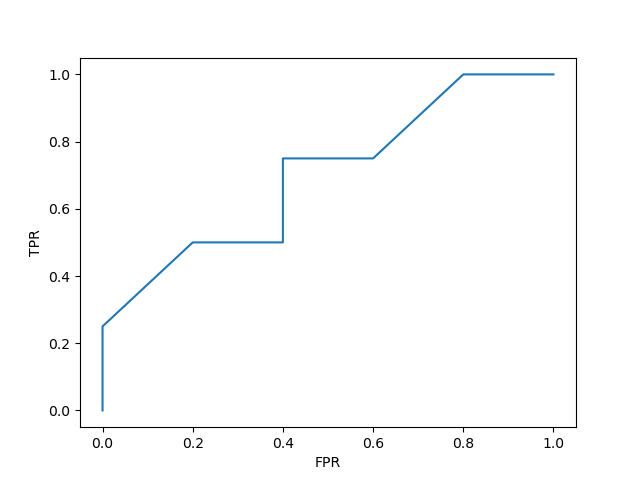
\includegraphics{roc1.jpg}
    \caption{ROC}
    \end{figure}
\newpage 
\item[(2)]
\begin{equation}
	\begin{aligned}
	AUC&= \frac{1}{2}\sum\limits_{i=1}^{7}(x_{i+1}-x_i)(y_{i+1}+y_i) \\
	   &= 0.075+0.1+0.15+0.175+0.2\\
	   &= 0.7 \\
	\end{aligned}
\end{equation}
\item[(3)]
根据AUC的计算公式可以得知,AUC是累加ROC曲线上相邻两个点与x轴围成的梯形的面积。

考虑点$(x_i, y_i)$和$(x_{i+1}, y_{i+1})$,若$x_i=x_{i+1}$则对应梯形的面积
为0.

假设$x_i\neq x_{i+1}$,即表示阈值变化后假正例率变大了,不妨考虑$x_{i+1}-x_i=\frac{1}{m^{-}}$
时的情况:

此时梯形较短的底边长度为:
\begin{equation}
	\sum\limits_{x^{+}\in D^{+}}(\frac{1}{m^{+}}\mathbb{I}\left\{f(x^{+})>f(x^{-})\right\})
\end{equation}
较长的底边长度为:
\begin{equation}
	\sum\limits_{x^{+}\in D^{+}}(\frac{1}{m^{+}}\mathbb{I}\left\{f(x^{+})>f(x^{-})\right\}+\frac{1}{m^{+}}\mathbb{I}\left\{f(x^{+})=f(x^{-})\right\})
\end{equation}
梯形的面积:
\begin{equation}
	\begin{aligned}
		S &= \frac{1}{2}(x_{i+1}-x_{i})\left[\sum\limits_{x^{+}\in D^{+}}(\frac{2}{m^{+}}\mathbb{I}\left\{f(x^{+})>f(x^{-})\right\}+\frac{1}{m^{+}}\mathbb{I}\left\{f(x^{+})=f(x^{-})\right\})\right] \\
		  &= \frac{1}{m^{+}m^{-}}\sum\limits_{x^{+}\in D^{+}}(\mathbb{I}\left\{f(x^{+})>f(x^{-})\right\}+\frac{1}{2}\mathbb{I}\left\{f(x^{+})=f(x^{-})\right\}) \\
	\end{aligned}
\end{equation}
因此,累加梯形的面积:
\begin{equation}
	\begin{aligned}
		AUC &= \sum\limits_{x^{-}\in D_{-}}S\\
		    &= \sum\limits_{x^{-}\in D_{-}}\frac{1}{m^{+}m^{-}}\sum\limits_{x^{+}\in D^{+}}(\mathbb{I}\left\{f(x^{+})>f(x^{-})\right\}+\frac{1}{2}\mathbb{I}\left\{f(x^{+})=f(x^{-})\right\})\\
			&= \frac{1}{m^{+}m^{-}}\sum\limits_{x^{+}\in D^{+}}\sum\limits_{x^{-}\in D^{-}}(\mathbb{I}\left\{f(x^{+})>f(x^{-})\right\}+\frac{1}{2}\mathbb{I}\left\{f(x^{+})=f(x^{-})\right\})\\
		\end{aligned}
\end{equation}
证毕。
\end{enumerate}
		~\\
		~\\
		~\\
	\end{solution}
	\newpage
	
	
	
	
	\section{[20pts] Linear Regression}
	线性回归模型是一类常见的机器学习方法, 其基础形式与变体常应用在回归任务中. 根据《机器学习》第三章 3.2 节中的定义, 可以将收集到的 $d$ 维数据及其标签如下表示: 
	
	\[
	\X=\left(\begin{array}{ccccc}
		x_{11} & x_{12} & \ldots & x_{1 d} & 1 \\
		x_{21} & x_{22} & \ldots & x_{2 d} & 1 \\
		\vdots & \vdots & \ddots & \vdots & \vdots \\
		x_{m 1} & x_{m 2} & \cdots & x_{m d} & 1
	\end{array}\right)
	=
	\left(\begin{array}{cc}
		\x_1^{\top} & 1 \\
		\x_2^{\top} & 1 \\
		\vdots & \vdots \\
		\x_m^{\top} & 1
	\end{array}\right)
	;\quad \y 
	=
	\left(\begin{array}{c}
		y_1\\
		y_2\\
		\vdots\\
		y_m
	\end{array}\right).
	\]
	
	将参数项与截距项合在一起, 定义为$\w=
	\left(
	\boldsymbol{w}^\top; b\right)^\top$. 此时成立 $\hat{\y} = \X\w$.《机器学习》式 (3.11) 给出了最小二乘估计 (Least Square Estimator, LSE) 的闭式解: 
	\begin{equation}
		\label{eq:LSE}
		\w_{\textbf{LSE}}^* = \left(\X^\top\X\right)^{-1}\X^\top\y.
	\end{equation}
	
	\begin{enumerate}
		\item[(1)] \textbf{[8pts]} (投影矩阵的性质) 
		% 在得到 $\w^*$ 后,可使用 $\mathbf{\hy} = \X \w^*$ 得到样本标记的预测值.
		容易验证, 当采用最小二乘估计 $\w_{\textbf{LSE}}^*$ 时, 成立: 
		\begin{equation*}
			\mathbf{\hy} = \X \w_{\textbf{LSE}}^* = \X\left(\X^\top\X\right)^{-1}\X^\top\y.
		\end{equation*}
		
		记 $\H = \X\left(\X^\top\X\right)^{-1}\X^\top$, 则有 $\mathbf{\hy} = \H\y$. $\H$ 被称为 “Hat Matrix”, 其存在可以从空间的角度, 把 $\mathbf{\hy}$ 看作是 $\y$ 在矩阵 $\H$ 空间中的投影. $\H$ 矩阵有着许多良好的性质.
		已知此时 $\X$ 矩阵列满秩, $\I$ 为单位阵, 试求 $\I - \H$ 的全部特征值并注明特征值的重数.
		% \begin{center}
			% \fcolorbox{gray}{gray!10}{\parbox{.85\linewidth}{背景: 记 $\H = \X\left(\X^\top\X\right)^{-1}\X^\top$,则有$\mathbf{\hy} = \H\y$.\\$\H$ 被称为“Hat Matrix”,其存在可以从空间的角度,把 $\mathbf{\hy}$ 看作是 $\y$ 在矩阵 $\H$ 空间中的投影.$\H$ 矩阵有着许多良好的性质.}}
			% \end{center}
		
		(提示: 利用 $\H$ 矩阵的投影性质与对称性.)
		
		
		
		\item[(2)] \textbf{[5pts]} (岭回归) 当数据量 $m$ 较小或数据维度 $d$ 较高时, 矩阵 $\X^\top\X$ 可能不满秩, \ref{eq:LSE} 中的取逆操作难以实现. 此时可使用岭回归代替原始回归问题, 其形式如下: 
		\begin{equation}
			\label{eq:Ridge}
			\w_{\textbf{Ridge}}^* = \mathop{\arg\min}_{\w} \frac{1}{2}\left(\lVert \y - \X \w \rVert_2^2 +\lambda \lVert \w \rVert_2^2\right).
		\end{equation}
		试求岭回归问题的闭式解, 并简述其对原问题的改进.
		
		\item[(3)] \textbf{[7pts]} 定义 $\Tilde{\x}_i = \left(\x_i^\top;1\right)^\top$,
		$\hy_i = \Tilde{\x}_i^\top \w_{\textbf{LSE}}^*$,
		$\by = \frac{1}{m} \sum\limits_{i=1}^m y_i $. 
		
		对线性回归模型进行统计分析时,会涉及如下三个基础定义: 
		\begin{equation*}
			\left\{
			\begin{aligned}
				&\text{Total sum of squares (SST): }& &\sum\limits_{i=1}^m\left(y_i-\by\right)^2 \\
				&\text{Regression sum of squares (SSR): }& &\sum\limits_{i=1}^m\left(\hy_i-y_i\right)^2 \\
				&\text{Residual sum of squares (SSE): }& &\sum\limits_{i=1}^m\left(\hy_i-\by\right)^2
			\end{aligned}
			\right.
		\end{equation*}
		
		试证明 SST = SSR + SSE. (提示: 使用向量形式可以简化证明步骤.)
		
		
		
	\end{enumerate}
	
	
	\begin{solution}
		此处用于写解答(中英文均可)
		\begin{enumerate}
			\item[(1)]
				$\because H^2=X(X^{T}X)^{-1}X^{T}X(X^{T}X)^{-1}X^{T}=X(X^{T}X)^{-1}X^{T}$

				$\therefore H$是幂等矩阵

				同理$(I-H)^2=I^{2}-2IH+H^{2}=I-2H+H=I-H$

				$\therefore I-H$也是幂等矩阵

				根据幂等矩阵的性质:$I-H$的特征值为0和1.

				$\because X$列满秩,$\therefore r(X)=d+1$

				$\therefore r(X^{T}X)=r(X)=d+1$

				$\therefore X^{T}X$是一个方阵且可逆

				又$\because X$列满秩,行满秩$\therefore r(H)=d+1$

				$\therefore I-H$的特征值为0(重数为d+1)和1(重数为m-d-1)
			\item[(2)] 
				\begin{equation}
					\begin{aligned}
						L(\w) &= \lVert \y - \X \w \rVert_2^2 +\lambda \lVert \w \rVert_2^2\\
										&= (\X\w-\y)^{T}(\X\w-\y) + \lambda \w^{T}\w \\
										&= \w^{T}\X^{T}\X\w-\y^{T}\X\w-\w^{T}X\y+y^{T}
					\end{aligned}
				\end{equation}
				所以:
				\begin{equation}
					\frac{\partial L(\w)}{\partial \w} = 2\X^{T}\X\w-2X^{T}y+2\lambda\w
				\end{equation}
				令$\frac{\partial L(\w)}{\partial \w}=0$,得:
				\begin{equation}
						\w=(\X^{T}\X+\lambda E)^{-1}\X^{T}\y 	
				\end{equation}
				岭回归在原问题得基础上增加了$L2$正则项$\lambda \w^{T}\w$,使得每个变量得权重不会太大。当
				某些特征权重比较大的时候,自变化变化一点,就会导致因变量变化很大,使得方差变大,有过拟合得
				风险。因此,岭回归在对局部特征较为明显的数据进行回归分析的时候有利于避
				免过拟合的现象,使得结果更为可靠。
			\item[(3)] 
				\begin{equation}
					\begin{aligned}
						SST &= \sum\limits_{i=1}^{m}(y_i-\by_i)^2 \\
							&= \sum\limits_{i=1}^{m}(y_i-\hy_i+\hy_i-\by_i)^2 \\
							&= \sum\limits_{i=1}^{m}(\hy_i-y_i)^2 + \sum\limits_{i=1}^{m}(\hy_i-\by_i)^2+2\sum\limits_{i=1}^{m}(y_i-\hy_i)(\hy_i-\by_i) \\
					\end{aligned}
				\end{equation}
				因此,欲证SST=SSR+SSE,只需证$\sum\limits_{i=1}^{m}(y_i-\hy_i)(\hy_i-\by_i)=0$
				
				已知$\hy_i = \Tilde{\x}_i^\top \w_{\textbf{LSE}}^*$
				因为采用最小二乘估计,所以
						$\frac{\partial E_{\w}}{\partial \w} = 2\X^{T}(\X\w-\y) = 0 $

						$\X\w-\y=0 $

						$\hy-\y = 0 $

				$\therefore \sum\limits_{i=1}^{m}(y_i-\hy_i)(\hy_i-\by_i)=0$

				SST=SSR+SSE,证毕。
		\end{enumerate}
		~\\
		~\\
		~\\
	\end{solution}
	
	\newpage
	\section{[35pts] Logistic Regression in Practice}
	对数几率回归 (Logistic Regression, 简称LR) 是实际应用中非常常用的分类学习算法.
	\begin{enumerate}
		\item[(1)]  \textbf{[30pts]} 请编程实现二分类的 LR, 要求采用牛顿法进行优化求解. 详细编程题指南请参见链接: \href{https://www.lamda.nju.edu.cn/ML2023Spring/homework/hw1/hw1-code.html}{here}. 请将绘制好的 ROC 曲线放在解答处, 并记录模型的精度与 AUC (保留4位小数).
		\item[(2)]  \textbf{[5pts]} 试简述在对数几率回归中, 相比梯度下降方法, 使用牛顿法的优点和缺点.
	\end{enumerate}
	
	\begin{solution}
		此处用于写解答 (中英文均可)
		~\\
		%%%%% use following code to insert the picture %%%%%
		\begin{enumerate}
			\item[(1)]如下图:
		
		\begin{figure}[H]
			\centering
			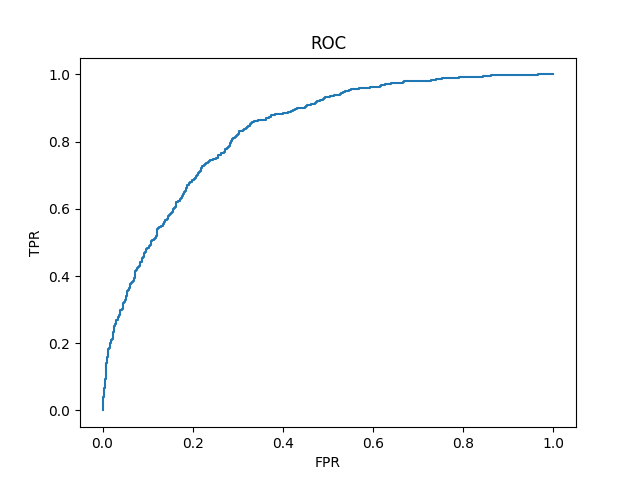
\includegraphics[width=0.8\textwidth]{Figure_1.png}\\
			\caption{ROC of test set}
			\label{fig:roc}
			\end{figure}
			
		模型精度:0.7621,AUC:0.8323
		\item[(2)]
		优点:牛顿迭代法只需进行二阶泰勒展开,收敛速度较快。

		缺点:1.涉及计算矩阵的逆,计算比较困难

		2.要求Hessian矩阵必须可逆

		3.局部收敛,若初始值$\w_0$选择不当可能会导致无法收敛
		\end{enumerate}
		~\\
		~\\
		~\\
	\end{solution}
	
	
	
\end{document}